% GNUPLOT: LaTeX picture with Postscript
\begingroup
  \makeatletter
  \providecommand\color[2][]{%
    \GenericError{(gnuplot) \space\space\space\@spaces}{%
      Package color not loaded in conjunction with
      terminal option `colourtext'%
    }{See the gnuplot documentation for explanation.%
    }{Either use 'blacktext' in gnuplot or load the package
      color.sty in LaTeX.}%
    \renewcommand\color[2][]{}%
  }%
  \providecommand\includegraphics[2][]{%
    \GenericError{(gnuplot) \space\space\space\@spaces}{%
      Package graphicx or graphics not loaded%
    }{See the gnuplot documentation for explanation.%
    }{The gnuplot epslatex terminal needs graphicx.sty or graphics.sty.}%
    \renewcommand\includegraphics[2][]{}%
  }%
  \providecommand\rotatebox[2]{#2}%
  \@ifundefined{ifGPcolor}{%
    \newif\ifGPcolor
    \GPcolortrue
  }{}%
  \@ifundefined{ifGPblacktext}{%
    \newif\ifGPblacktext
    \GPblacktextfalse
  }{}%
  % define a \g@addto@macro without @ in the name:
  \let\gplgaddtomacro\g@addto@macro
  % define empty templates for all commands taking text:
  \gdef\gplbacktext{}%
  \gdef\gplfronttext{}%
  \makeatother
  \ifGPblacktext
    % no textcolor at all
    \def\colorrgb#1{}%
    \def\colorgray#1{}%
  \else
    % gray or color?
    \ifGPcolor
      \def\colorrgb#1{\color[rgb]{#1}}%
      \def\colorgray#1{\color[gray]{#1}}%
      \expandafter\def\csname LTw\endcsname{\color{white}}%
      \expandafter\def\csname LTb\endcsname{\color{black}}%
      \expandafter\def\csname LTa\endcsname{\color{black}}%
      \expandafter\def\csname LT0\endcsname{\color[rgb]{1,0,0}}%
      \expandafter\def\csname LT1\endcsname{\color[rgb]{0,1,0}}%
      \expandafter\def\csname LT2\endcsname{\color[rgb]{0,0,1}}%
      \expandafter\def\csname LT3\endcsname{\color[rgb]{1,0,1}}%
      \expandafter\def\csname LT4\endcsname{\color[rgb]{0,1,1}}%
      \expandafter\def\csname LT5\endcsname{\color[rgb]{1,1,0}}%
      \expandafter\def\csname LT6\endcsname{\color[rgb]{0,0,0}}%
      \expandafter\def\csname LT7\endcsname{\color[rgb]{1,0.3,0}}%
      \expandafter\def\csname LT8\endcsname{\color[rgb]{0.5,0.5,0.5}}%
    \else
      % gray
      \def\colorrgb#1{\color{black}}%
      \def\colorgray#1{\color[gray]{#1}}%
      \expandafter\def\csname LTw\endcsname{\color{white}}%
      \expandafter\def\csname LTb\endcsname{\color{black}}%
      \expandafter\def\csname LTa\endcsname{\color{black}}%
      \expandafter\def\csname LT0\endcsname{\color{black}}%
      \expandafter\def\csname LT1\endcsname{\color{black}}%
      \expandafter\def\csname LT2\endcsname{\color{black}}%
      \expandafter\def\csname LT3\endcsname{\color{black}}%
      \expandafter\def\csname LT4\endcsname{\color{black}}%
      \expandafter\def\csname LT5\endcsname{\color{black}}%
      \expandafter\def\csname LT6\endcsname{\color{black}}%
      \expandafter\def\csname LT7\endcsname{\color{black}}%
      \expandafter\def\csname LT8\endcsname{\color{black}}%
    \fi
  \fi
  \setlength{\unitlength}{0.0500bp}%
  \begin{picture}(8502.00,2834.00)%
    \gplgaddtomacro\gplbacktext{%
      \csname LTb\endcsname%
      \put(1210,918){\makebox(0,0)[r]{\strut{}\scriptsize -0.3}}%
      \put(1210,1158){\makebox(0,0)[r]{\strut{}\scriptsize -0.2}}%
      \put(1210,1397){\makebox(0,0)[r]{\strut{}\scriptsize -0.1}}%
      \put(1210,1636){\makebox(0,0)[r]{\strut{}\scriptsize 0}}%
      \put(1210,1876){\makebox(0,0)[r]{\strut{}\scriptsize 0.1}}%
      \put(1210,2115){\makebox(0,0)[r]{\strut{}\scriptsize 0.2}}%
      \put(1210,2355){\makebox(0,0)[r]{\strut{}\scriptsize 0.3}}%
      \put(1397,484){\makebox(0,0){\strut{}\scriptsize -0.4}}%
      \put(1742,484){\makebox(0,0){\strut{}\scriptsize -0.2}}%
      \put(2088,484){\makebox(0,0){\strut{}\scriptsize 0}}%
      \put(2434,484){\makebox(0,0){\strut{}\scriptsize 0.2}}%
      \put(2779,484){\makebox(0,0){\strut{}\scriptsize 0.4}}%
      \put(176,1636){\rotatebox{-270}{\makebox(0,0){\strut{}$u_{R}$ (\AA)}}}%
      \put(2088,154){\makebox(0,0){\strut{}$u_{ir}$ (\AA)}}%
      \put(1105,2720){\makebox(0,0)[l]{\strut{}$\lambda_{ir} = 0.00$ eV}}%
    }%
    \gplgaddtomacro\gplfronttext{%
    }%
    \gplgaddtomacro\gplbacktext{%
      \csname LTb\endcsname%
      \put(3088,918){\makebox(0,0)[r]{\strut{}}}%
      \put(3088,1158){\makebox(0,0)[r]{\strut{}}}%
      \put(3088,1397){\makebox(0,0)[r]{\strut{}}}%
      \put(3088,1636){\makebox(0,0)[r]{\strut{}}}%
      \put(3088,1876){\makebox(0,0)[r]{\strut{}}}%
      \put(3088,2115){\makebox(0,0)[r]{\strut{}}}%
      \put(3088,2355){\makebox(0,0)[r]{\strut{}}}%
      \put(3288,484){\makebox(0,0){\strut{}\scriptsize -0.4}}%
      \put(3721,484){\makebox(0,0){\strut{}\scriptsize -0.2}}%
      \put(4154,484){\makebox(0,0){\strut{}\scriptsize 0}}%
      \put(4586,484){\makebox(0,0){\strut{}\scriptsize 0.2}}%
      \put(5019,484){\makebox(0,0){\strut{}\scriptsize 0.4}}%
      \put(3066,1636){\rotatebox{-270}{\makebox(0,0){\strut{}}}}%
      \put(4153,154){\makebox(0,0){\strut{}$u_{ir}$ (\AA)}}%
      \put(3400,2720){\makebox(0,0)[l]{\strut{}$\lambda_{ir} = 0.1263$ eV}}%
    }%
    \gplgaddtomacro\gplfronttext{%
    }%
    \gplgaddtomacro\gplbacktext{%
      \csname LTb\endcsname%
      \put(5681,918){\makebox(0,0)[r]{\strut{}}}%
      \put(5681,1158){\makebox(0,0)[r]{\strut{}}}%
      \put(5681,1397){\makebox(0,0)[r]{\strut{}}}%
      \put(5681,1636){\makebox(0,0)[r]{\strut{}}}%
      \put(5681,1876){\makebox(0,0)[r]{\strut{}}}%
      \put(5681,2115){\makebox(0,0)[r]{\strut{}}}%
      \put(5681,2355){\makebox(0,0)[r]{\strut{}}}%
      \put(5872,484){\makebox(0,0){\strut{}\scriptsize -0.4}}%
      \put(6246,484){\makebox(0,0){\strut{}\scriptsize -0.2}}%
      \put(6620,484){\makebox(0,0){\strut{}\scriptsize 0}}%
      \put(6994,484){\makebox(0,0){\strut{}\scriptsize 0.2}}%
      \put(7368,484){\makebox(0,0){\strut{}\scriptsize 0.4}}%
      \put(5659,1636){\rotatebox{-270}{\makebox(0,0){\strut{}}}}%
      \put(6620,154){\makebox(0,0){\strut{}$u_{ir}$ (\AA)}}%
      \put(5951,2720){\makebox(0,0)[l]{\strut{}$\lambda_{ir} = 0.25$ eV}}%
    }%
    \gplgaddtomacro\gplfronttext{%
      \csname LTb\endcsname%
      \put(7679,704){\makebox(0,0)[l]{\strut{} 0}}%
      \put(7679,1014){\makebox(0,0)[l]{\strut{} 0.02}}%
      \put(7679,1325){\makebox(0,0)[l]{\strut{} 0.04}}%
      \put(7679,1636){\makebox(0,0)[l]{\strut{} 0.06}}%
      \put(7679,1947){\makebox(0,0)[l]{\strut{} 0.08}}%
      \put(7679,2258){\makebox(0,0)[l]{\strut{} 0.1}}%
      \put(7679,2569){\makebox(0,0)[l]{\strut{} 0.12}}%
    }%
    \gplbacktext
    \put(0,0){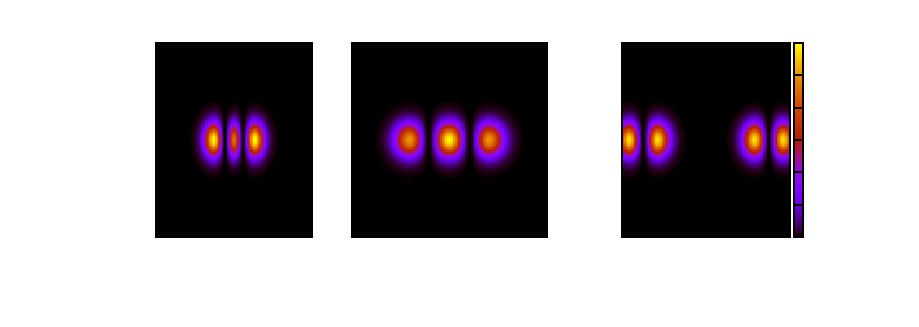
\includegraphics{images/phononProj2ir}}%
    \gplfronttext
  \end{picture}%
\endgroup
